\documentclass[12pt,letterpaper]{article}
\usepackage[utf8]{inputenc}
\usepackage[spanish]{babel}
\usepackage{graphicx}
\usepackage[left=2cm,right=2cm,top=2cm,bottom=2cm]{geometry}
\usepackage{graphicx} % figuras
% \usepackage{subfigure} % subfiguras
\usepackage{float} % para usar [H]
\usepackage{amsmath}
%\usepackage{txfonts}
\usepackage{stackrel} 
\usepackage{multirow}
\usepackage{enumerate} % enumerados
\renewcommand{\labelitemi}{$-$}
\renewcommand{\labelitemii}{$\cdot$}
% \author{}
% \title{Caratula}
\begin{document}

% Fancy Header and Footer
% \usepackage{fancyhdr}
% \pagestyle{fancy}
% \cfoot{}
% \rfoot{\thepage}
%

% \usepackage[hidelinks]{hyperref} % CREA HYPERVINCULOS EN INDICE

% \author{}
\title{Caratula}

\begin{titlepage}
\begin{center}
\large{UNERSIDAD PRIVADA DE TACNA}\\
\vspace*{-0.025in}
\begin{figure}[htb]
\begin{center}

\includegraphics[width=8cm]{imagenes/logo.jpg}
\end{center}
\end{figure}
\vspace*{0.15in}
INGENIERIA DE SISTEMAS  \\

\vspace*{0.5in}
\begin{large}
TITULO:\\
\end{large}

\vspace*{0.1in}
\begin{Large}
\textbf{INFORME DE LABORATORIO No 04} \\
\end{Large}

\vspace*{0.3in}
\begin{Large}
\textbf{CURSO:} \\
\end{Large}

\vspace*{0.1in}
\begin{large}
INTELIGENCIA DE NEGOCIOS\\
\end{large}

\vspace*{0.3in}
\begin{Large}
\textbf{DOCENTE(ING):} \\
\end{Large}

\vspace*{0.1in}
\begin{large}
 Patrick Cuadros Quiroga\\
\end{large}

\vspace*{0.2in}
\vspace*{0.1in}
\begin{large}
Alumna: \\
\begin{flushleft}
Layme Valeriano Diego Rolando		\hfill	(2017057865) \\
\end{flushleft}
\end{large}
\end{center}

\end{titlepage}


\tableofcontents % INDICE
\thispagestyle{empty} % INDICE SIN NUMERO
\newpage
\setcounter{page}{1} % REINICIAR CONTADOR DE PAGINAS DESPUES DEL INDICE

\section{Ejercicio 1}
\textbf{MODELO FISICO}\\\\
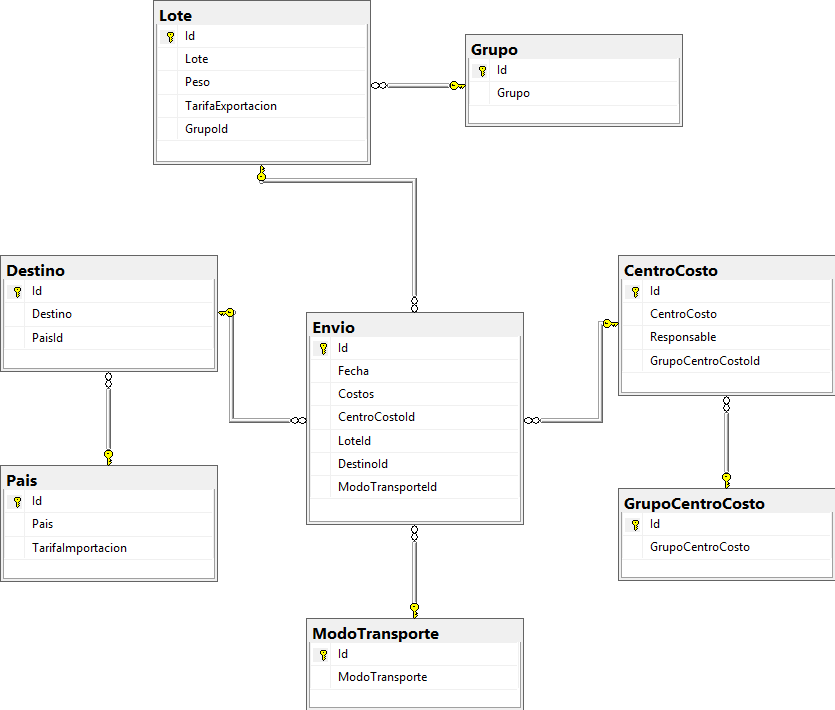
\includegraphics[width=14cm,height=10cm,keepaspectratio]{imagenes/e1.png}\\
\newpage
\textbf{MODELO DIMENSIONAL}\\\\
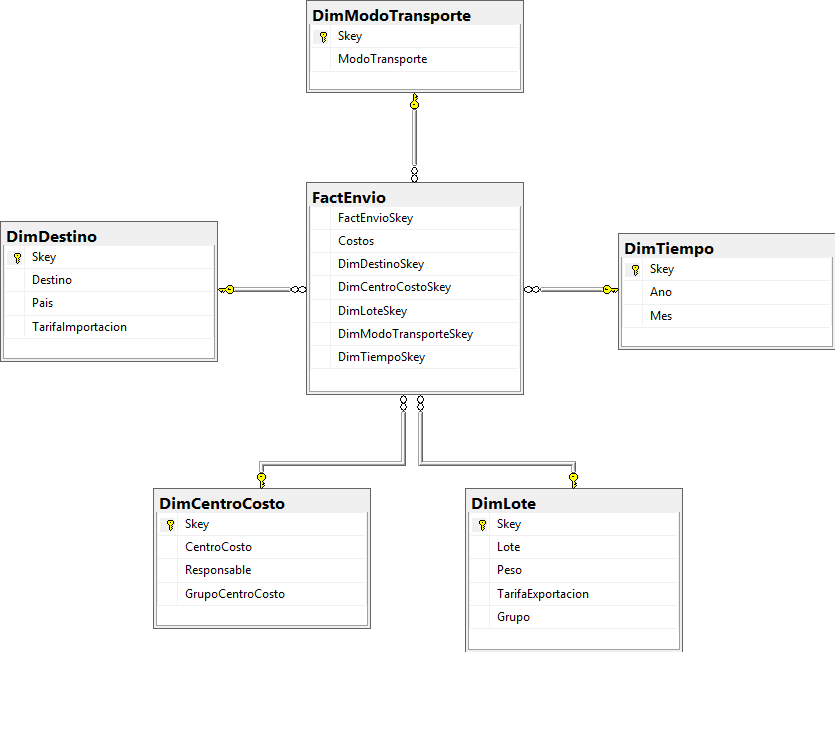
\includegraphics[width=14cm]{imagenes/d1.png}\\

\newpage
\section{Ejercicio 2}
\textbf{MODELO FISICO}\\\\
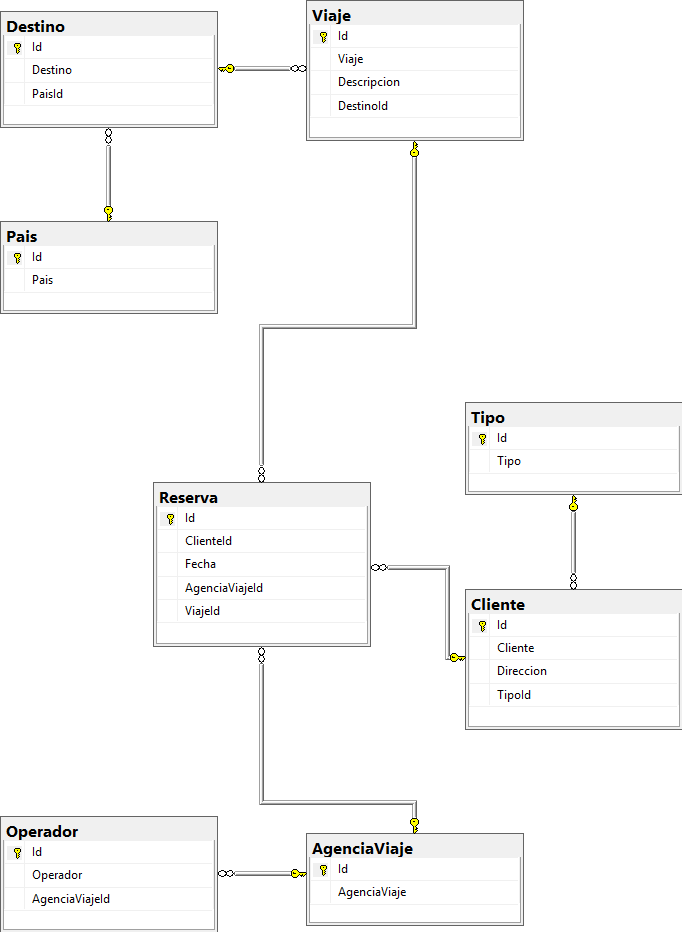
\includegraphics[width=14cm]{imagenes/e2.png}\\
\newpage
\textbf{MODELO DIMENSIONAL}\\\\
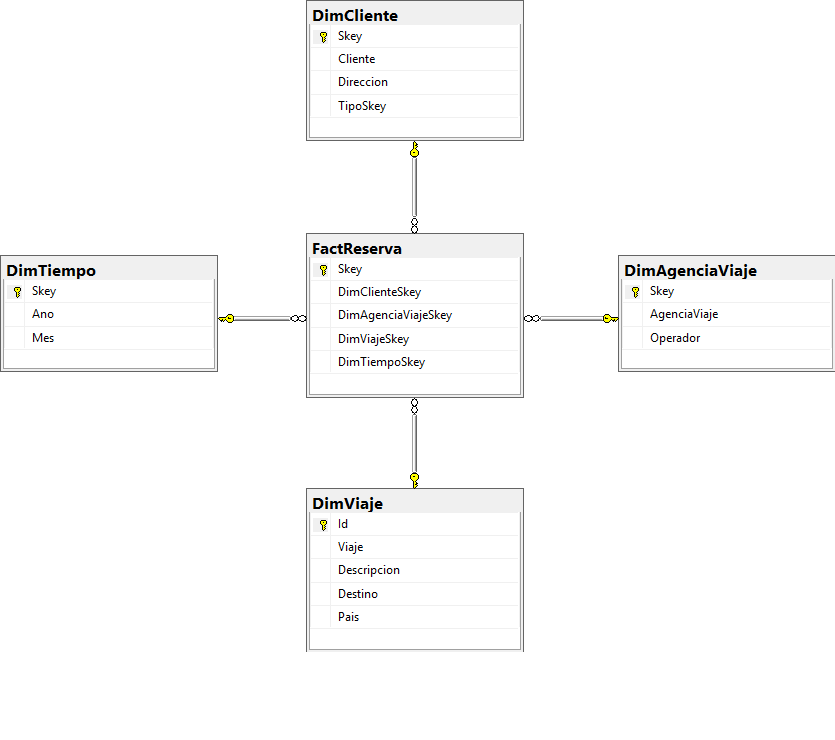
\includegraphics[width=14cm]{imagenes/d2.png}\\

\newpage
\section{Ejercicio 3}
\textbf{MODELO FISICO}\\\\
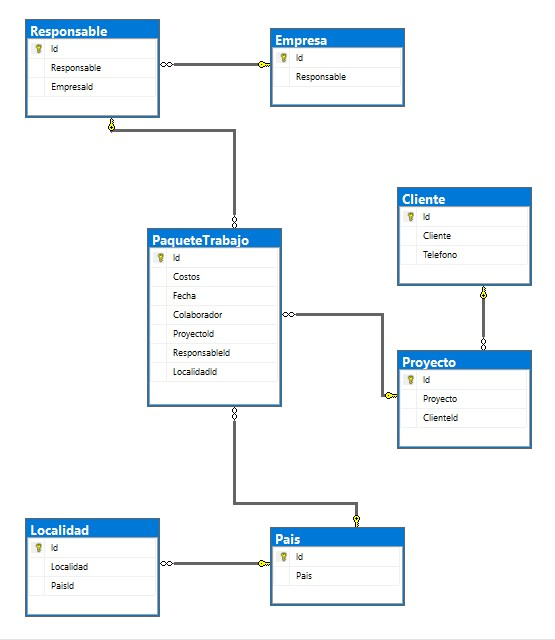
\includegraphics[width=14cm]{imagenes/e3.jpg}\\
\newpage
\textbf{MODELO DIMENSIONAL}\\\\
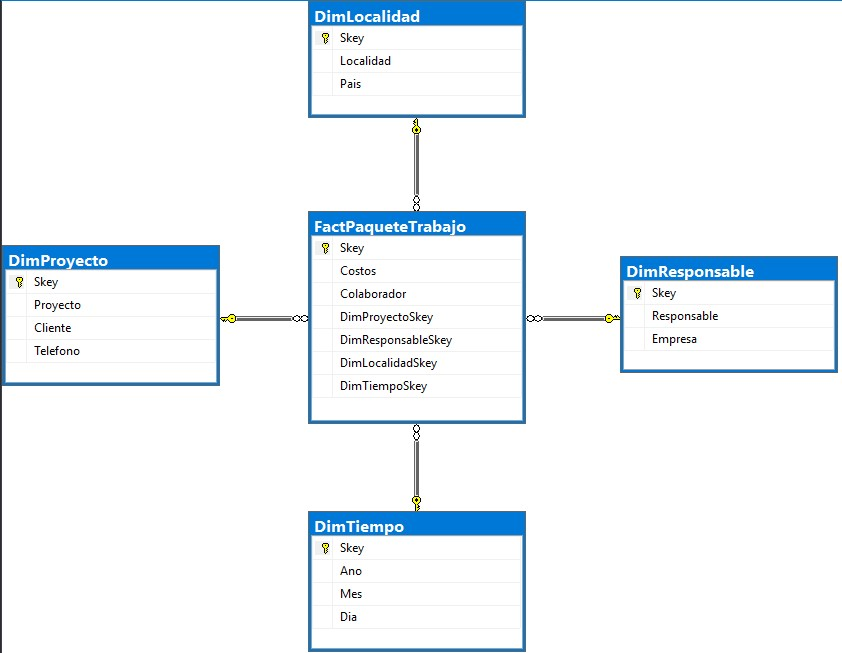
\includegraphics[width=14cm]{imagenes/d3.jpg}\\

\end{document}
